\newpage
\subsubsection{Drehräder-Modell}
\begin{figure}[h!]
	\centering
	\begin{subfigure}{.4\textwidth}
		\centering
		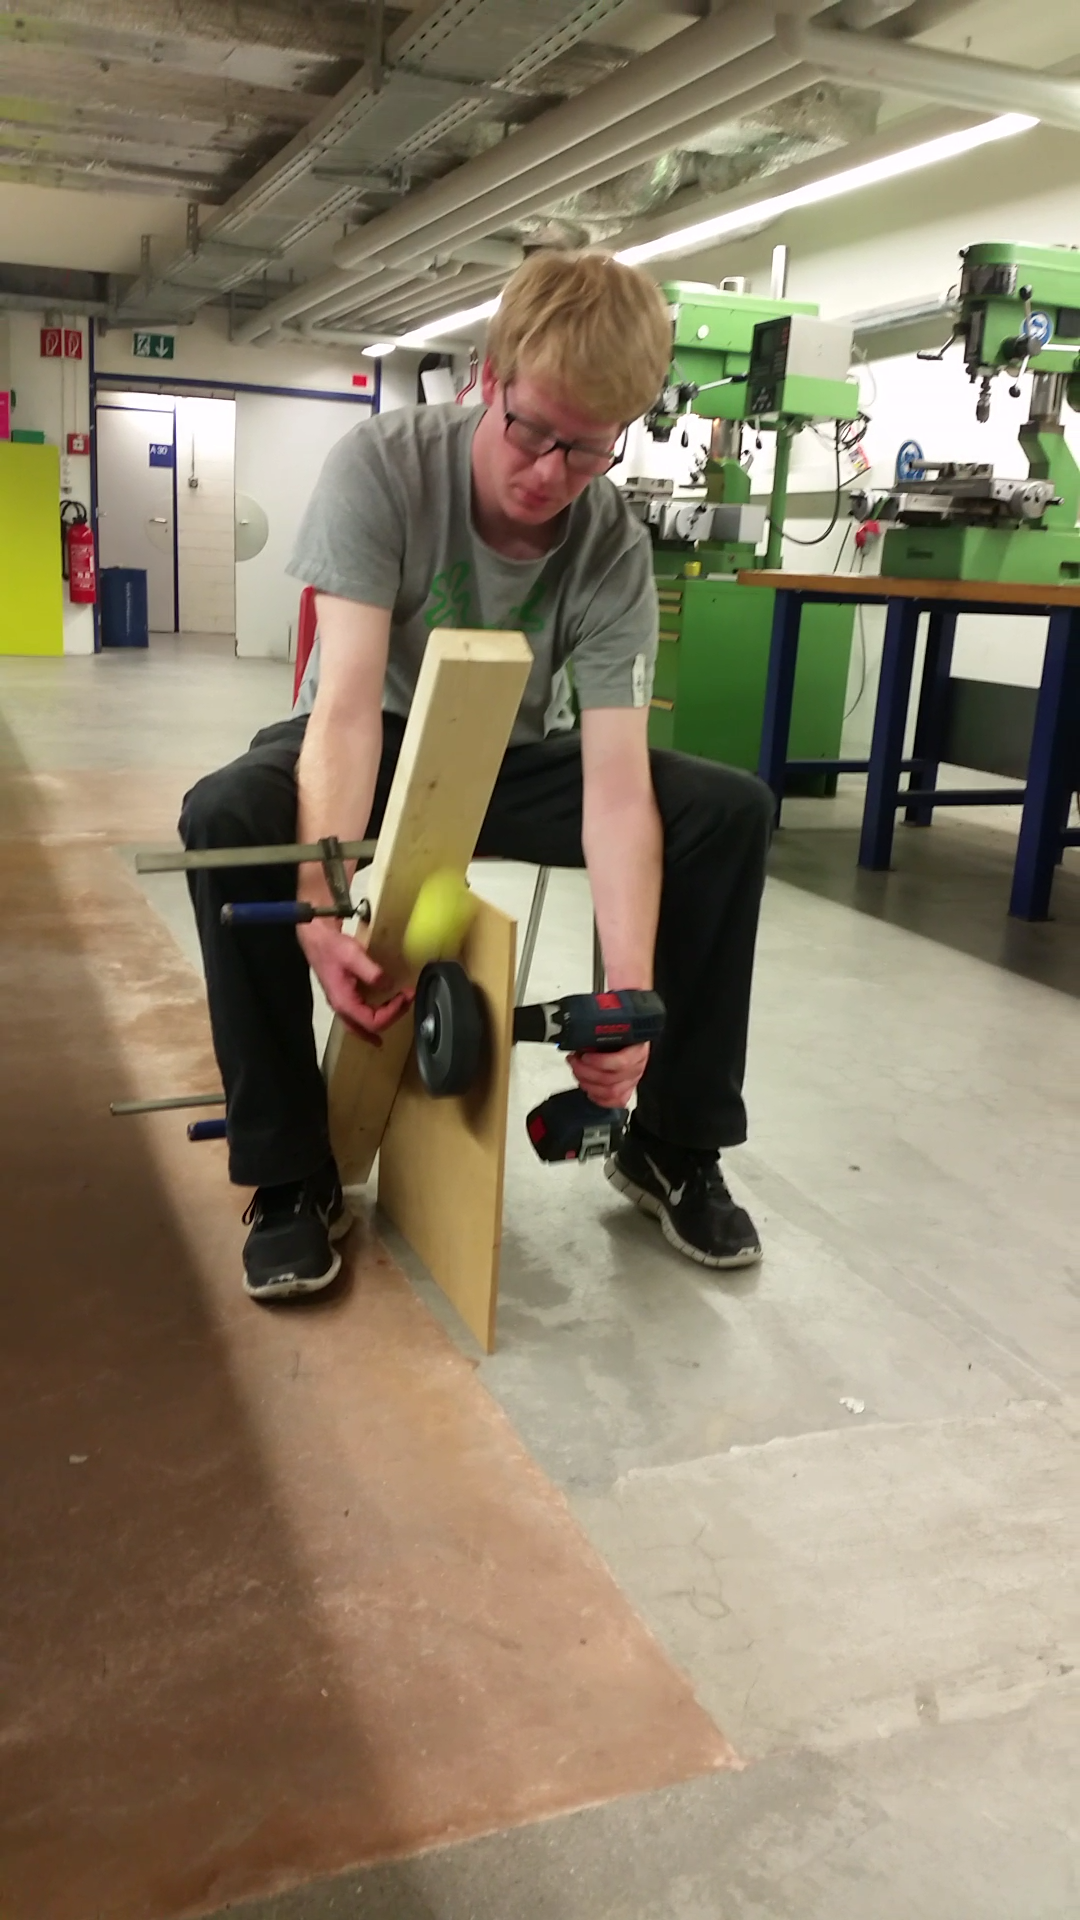
\includegraphics[width=0.6\textwidth]{../../fig/Versuch_Drehrad.png}
		\caption{Schrägen Wurf von der Seite}
		\label{fig:Aufbau der Versuch}
	\end{subfigure} %
	\begin{subfigure}{.4\textwidth}
		\centering
		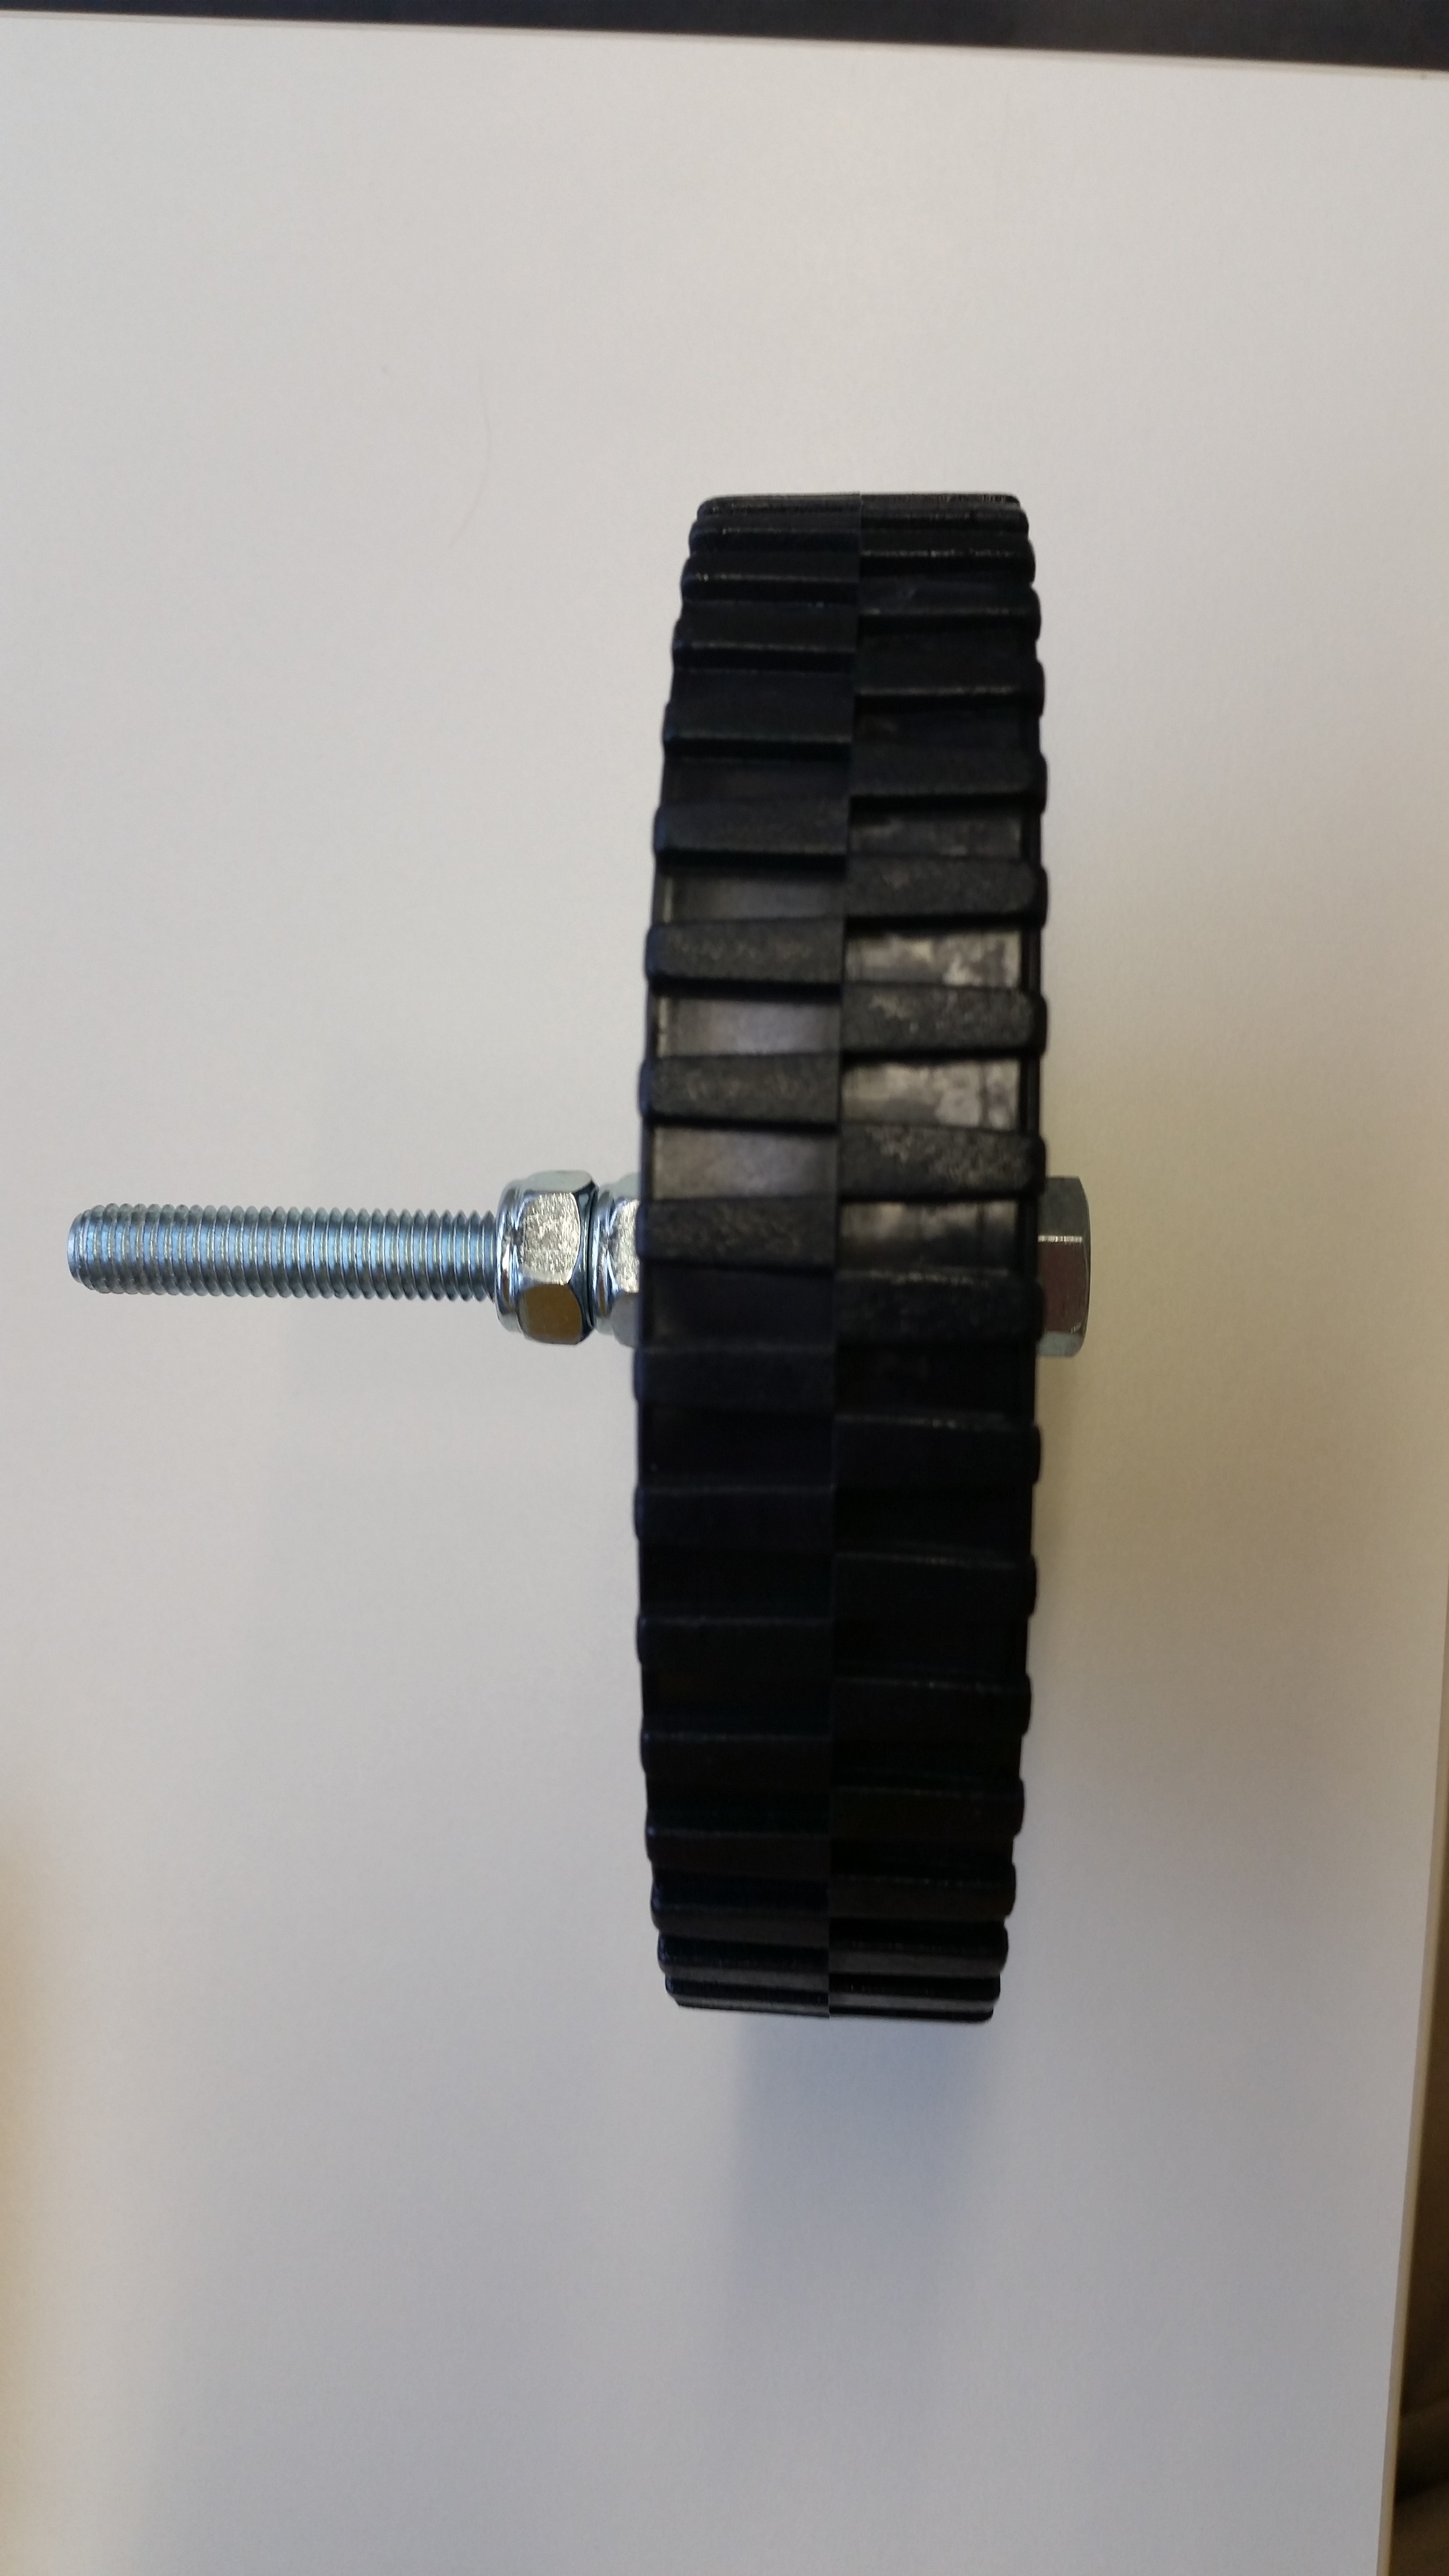
\includegraphics[width=0.6\textwidth]{../../fig/Drehrad_1.jpg}
		\caption{Schrägen Wurf von Oben}
		\label{fig:Drehrad}
	\end{subfigure}
	\caption{Berechnung der Schräger Wurf}
	\label{Drehrad Versuch}
\end{figure}
Wir haben einen 15 cm Durchmesser Drehrad aus PVC benutzt um einem Prototyp unseres Wurfmaschine  aufzubauen. Als Betriebsmotor haben wir ein Akkubohrermaschine benutzt.
Mit ein kleines Aufbau haben wir versucht die Regelmässigkeit zu testen. Es war uns nicht wichtig ob die genaue Distanz erreicht wurde, sonst nur ob es bei jedem Schuss immer auf der selbe Abstand war. Mit der Versuch sollte auch nachgeschaut werden, was für eine Auswirkung der Drehung der Ball haben könnte. Der Versuch wurde in 2 Arten gemacht: ein erstes mal mit der Drehrad oben der Ball, und ein zweites mit der Drehrad unten. Mit diesem Unterschied es ist möglich der Auswirkung der Drehung der Ball zu festlegen und auch welche Vorrichtung einem besserem Schuss geben kann.\\ \\
Nach mehrere versuche wurde festgelegt das es ein sehr Regelmässiges system ist, auch wenn der Prototyp nicht so stabil war wie wir gedacht haben. Der Wurf hat 1.3 Meter erreicht und alle Bälle sind innerhalb einem Kreis mit einem Durchmesser kleiner als 30 cm gelandet. Mit einige Anpassungen die an die Maschine gemacht werden können, wie zum Beispiel eine genauere Vorrichtung und ein Rad aus weicheres Material, kann die Genauigkeit noch erhöht werden.\\ Als weiteres haben wir bemerkt das der Wurf mit der Drehrad Unter der Ball etwas präziser ist. Weiterhin haben wir notiert das der Drehung der Ball keine Auswirkung auf der Flugbahn hat. Das wurde erwartet, da die Geschwindigkeit der Wurf und der Drehung klein ist. \\

